% \section{Method}
% \label{sec:method}

\subsection{\ours Overview}
\label{sec:overview}

\begin{figure*}[t]
    \centering
    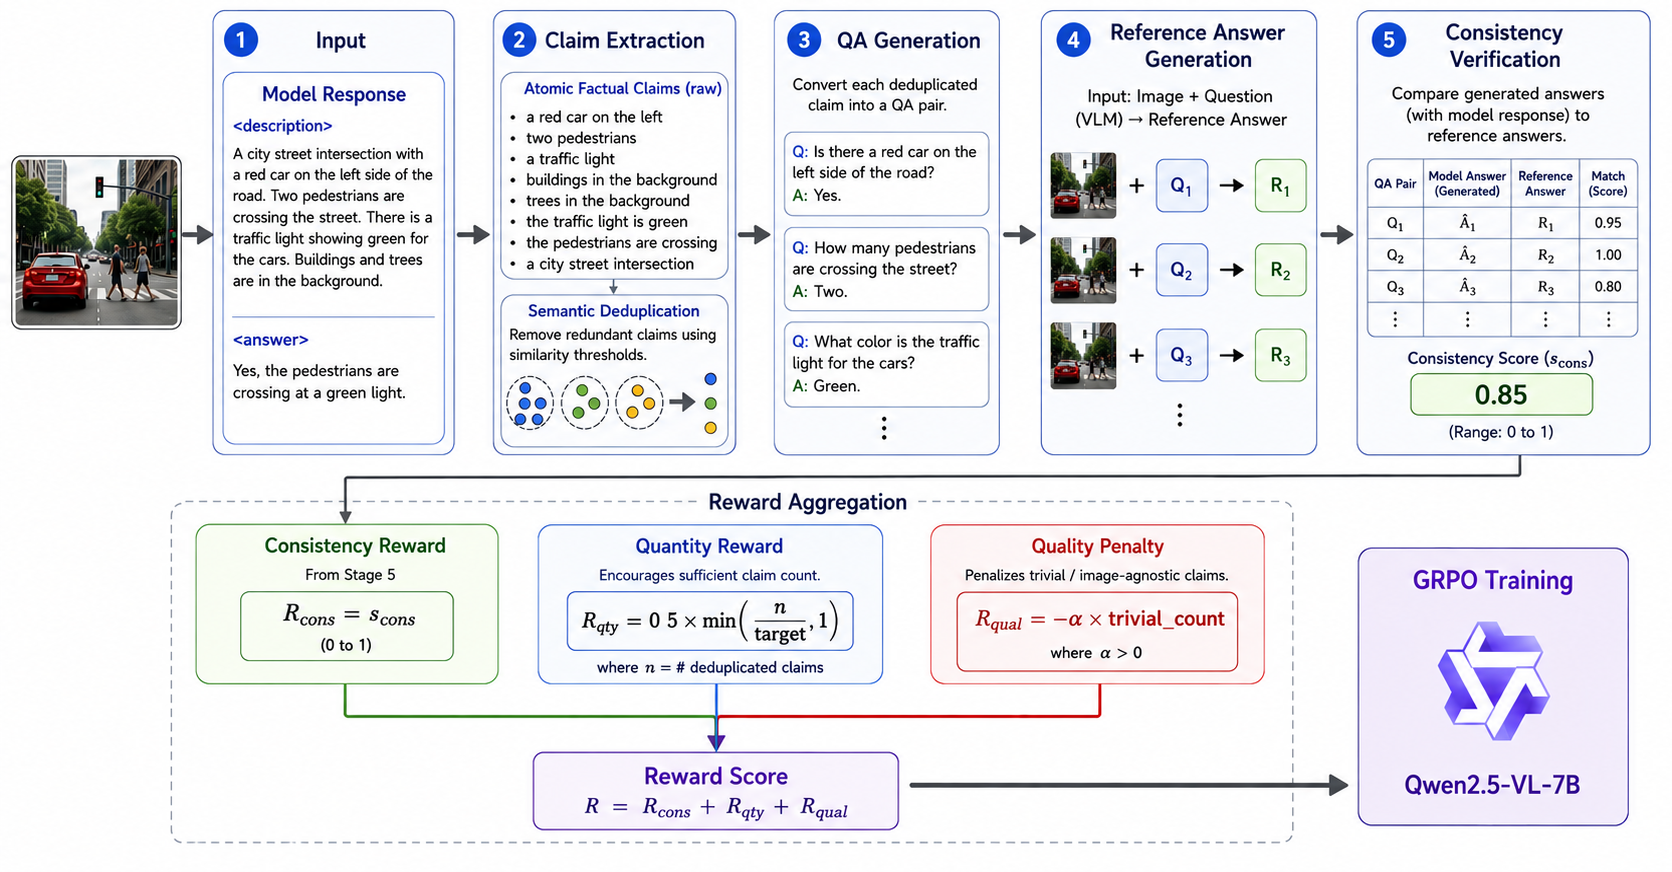
\includegraphics[width=\textwidth]{figures/pipeline.png}
    \caption{Overview of the \ours pipeline. Given a model-generated response,
    the Proposer decomposes the description into atomic factual claims and
    removes semantically redundant claims. Each remaining claim is converted into
    a visual question-answer pair. The Checker answers the question using only
    the input image, without observing the original description. The implied
    answer and the image-grounded answer are compared to produce claim-level
    verification signals. Finally, \ours aggregates consistency reward,
    informativeness reward, and visual evidence calibration penalty into a scalar
    reward for GRPO training.}
    \label{fig:pipeline}
\end{figure*}

The key idea of \ours is to transform open-ended visual factuality evaluation into a set of fine-grained, image-grounded verification problems. 
Instead of asking a model to holistically judge whether an entire response is correct, we first decompose the generated description into atomic claims and verify each claim independently against the image.

As shown in Fig.~\ref{fig:pipeline}, \ours consists of three conceptual stages.
First, a \textit{Proposer} agent extracts atomic factual claims from $y^{\mathrm{desc}}$ and converts them into visual question-answer pairs. 
Second, a \textit{Checker} agent answers each question using only the input image $I$, without access to the original model description. 
Third, the system compares the answer implied by the generated description with the image-grounded answer and aggregates the resulting claim-level scores into a scalar reward.

This asymmetric design is crucial. If the same model verifies a claim while seeing the generated description, it may simply confirm the textual prior rather than inspect the image, leading to self-confirmation bias. 
In contrast, the Checker in \ours only observes the image and the verification question. This information asymmetry forces verification to rely on visual evidence instead of the original generated text.

\subsection{Asymmetric Claim-Level Verification}
\label{sec:claim_verification}

\paragraph{Claim Proposal.}
Given a generated description $y^{\mathrm{desc}}$, the Proposer extracts a set
of atomic factual claims:
\begin{equation}
    \mathcal{C}
    =
    \{c_1,c_2,\ldots,c_m\}
    =
    \mathrm{Prop}(y^{\mathrm{desc}}).
\end{equation}
Each claim $c_i$ is a short and self-contained statement about a single visual
fact, such as object existence, color, quantity, action, or spatial relation.
For example, from the description
\textit{``A red car is parked on the left side of the road''}, the Proposer may
extract claims such as \textit{``there is a car''}, \textit{``the car is red''},
and \textit{``the car is on the left side of the road''}. This decomposition
turns a long-form description into independently verifiable factual units.

\paragraph{Semantic Deduplication.}
Directly rewarding all extracted claims may encourage verbosity and repetition:
a model could repeat the same correct fact multiple times to inflate the reward.
To prevent this reward hacking behavior, we deduplicate claims before
verification. Each claim $c_i$ is encoded by a sentence encoder $\phi(\cdot)$,
and pairwise semantic similarity is computed as
\begin{equation}
    \mathrm{sim}(c_i,c_j)
    =
    \frac{
    \phi(c_i)^\top \phi(c_j)
    }{
    \|\phi(c_i)\| \cdot \|\phi(c_j)\|
    }.
\end{equation}
If $\mathrm{sim}(c_i,c_j)>\tau$, the two claims are treated as duplicates, and
only one representative is retained. We denote the deduplicated claim set as
\begin{equation}
    \mathcal{C}^{\ast}
    =
    \{c_1^{\ast},c_2^{\ast},\ldots,c_n^{\ast}\},
\end{equation}
where $n \leq m$. This ensures that the reward reflects the diversity of visual
facts rather than the length of the response.

\paragraph{Question-Answer Transformation.}
For each deduplicated claim $c_i^{\ast}$, the Proposer constructs a visual
question-answer pair:
\begin{equation}
    (v_i,\hat{a}_i)
    =
    \mathrm{QA}(c_i^{\ast}),
\end{equation}
where $v_i$ is a visual question and $\hat{a}_i$ is the answer implied by the
claim. For instance, the claim \textit{``the traffic light is green''} can be
converted into the question \textit{``What color is the traffic light?''} with
the implied answer \textit{``green''}. This step converts declarative factual
claims into a format that can be checked independently from the original
description.

\paragraph{Image-Grounded Checking.}
The Checker answers each verification question using the original image:
\begin{equation}
    a_i =
    \mathrm{Check}(I,v_i).
\end{equation}
Importantly, the Checker does not observe $y^{\mathrm{desc}}$ or $c_i^{\ast}$.
It only receives the image $I$ and the question $v_i$. Therefore, $a_i$ serves as
an image-grounded reference answer, while $\hat{a}_i$ represents the answer
implied by the generated description.

\paragraph{Consistency Reward.}
We compare $\hat{a}_i$ and $a_i$ with a soft matching function
$f_{\mathrm{match}}(\cdot,\cdot)$, which accounts for lexical variants and
semantically equivalent answers. The consistency reward is defined as
\begin{equation}
    R_{\mathrm{cons}}
    =
    \frac{1}{n}
    \sum_{i=1}^{n}
    f_{\mathrm{match}}(\hat{a}_i,a_i),
\end{equation}
where $R_{\mathrm{cons}}\in[0,1]$. This term directly measures whether the
visual claims in the model-generated description are supported by the image.

\subsection{Visual Evidence Calibration}
\label{sec:vec}

While claim-level consistency provides fine-grained supervision, it is still
vulnerable to degenerate strategies. A model may produce overly generic claims
that are easy to verify, or repeat high-confidence but low-information facts.
Such claims can obtain high consistency scores without improving genuine visual
grounding. To address this, we introduce \textit{Visual Evidence Calibration}
(VEC), which calibrates the self-verifying reward along two dimensions:
informativeness and visual dependence.

\paragraph{Informativeness Reward.}
A factual description should contain a sufficient number of distinct visual
claims. To encourage informative descriptions, we introduce a quantity-based
reward:
\begin{equation}
    R_{\mathrm{info}}
    =
    \lambda_{\mathrm{info}}
    \cdot
    \min
    \left(
        \frac{n}{n_{\mathrm{target}}},
        1
    \right),
\end{equation}
where $n$ is the number of deduplicated claims,
$n_{\mathrm{target}}$ is the target number of distinct claims, and
$\lambda_{\mathrm{info}}$ controls the maximum contribution of this term. This
reward is capped so that factual consistency remains the dominant optimization
signal.

\paragraph{Visual Dependence Penalty.}
Some claims are answerable without meaningful visual inspection. For example,
generic statements such as \textit{``there are objects in the image''} may be
correct for most images and thus provide little grounding signal. To identify
such image-agnostic claims, we use a degraded visual input $\tilde{I}$, obtained
by heavily blurring the original image. The Checker answers the same question
$v_i$ using $\tilde{I}$:
\begin{equation}
    \tilde{a}_i =
    \mathrm{Check}(\tilde{I},v_i).
\end{equation}
If the implied answer $\hat{a}_i$ still matches the answer obtained from the
blurred image, the claim is considered weakly dependent on visual evidence:
\begin{equation}
    \mathbbm{1}_{\mathrm{triv}}(i)
    =
    \mathbbm{1}
    \left[
        f_{\mathrm{match}}(\hat{a}_i,\tilde{a}_i)>\delta
    \right],
\end{equation}
where $\delta$ is a matching threshold. The visual dependence penalty is then
defined as
\begin{equation}
    R_{\mathrm{dep}}
    =
    -
    \lambda_{\mathrm{dep}}
    \sum_{i=1}^{n}
    \mathbbm{1}_{\mathrm{triv}}(i),
\end{equation}
where $\lambda_{\mathrm{dep}}>0$ controls the penalty strength. This term
discourages claims that can be verified without sufficient visual evidence.

\subsection{Reward Aggregation and Policy Optimization}
\label{sec:reward_aggregation}

The final self-verifying reward used for GRPO training combines claim-level
consistency with the VEC calibration terms:
\begin{equation}
    R_{\mathrm{SV}}(I,q,y)
    =
    R_{\mathrm{cons}}
    +
    R_{\mathrm{info}}
    +
    R_{\mathrm{dep}}.
\end{equation}
We use this reward as the scalar RL reward:
\begin{equation}
    r(I,q,y)
    =
    R_{\mathrm{SV}}(I,q,y).
\end{equation}

The three components play complementary roles. $R_{\mathrm{cons}}$ encourages
the generated description to be factually consistent with the image;
$R_{\mathrm{info}}$ prevents the model from producing overly short or
uninformative descriptions; and $R_{\mathrm{dep}}$ suppresses claims that are
trivially answerable without genuine visual grounding. Together, they provide a
dense and scalable reward signal for hallucination mitigation without requiring
human-annotated captions or ground-truth factual labels.

During training, for each input image-instruction pair $(I,q)$, we sample a group
of responses from the current policy, compute $R_{\mathrm{SV}}$ for each
response through the asymmetric verification pipeline, normalize the rewards
within the group to obtain GRPO advantages, and update the policy using
$\mathcal{L}_{\mathrm{GRPO}}$. This completes an annotation-free RLVR loop in
which the model improves its visual factuality through self-generated,
image-grounded verification signals.
